\subsection{Effect of varying $\tau_h$ and $\tau_r$}
The bit that is sent through the transmission line model is defined by the rising time ($\tau_r$) and a bit time ($T_{bit} = \tau_h$). A falling time ($\tau_f$) could be defined, but a symmetrical bit is assumed so $\tau_r = \tau_f$. The default settings are $\tau_h = 100*10^{-12}$ and $\tau_r = 40*10^{-12}$. For this values, the bit has a trapezium shape. This case is shown in figure~\ref{fig:default} Letting these values vary a bit, one discovers a few interesting cases worth it to have look at.

\begin{figure}[h!]
    \centering
    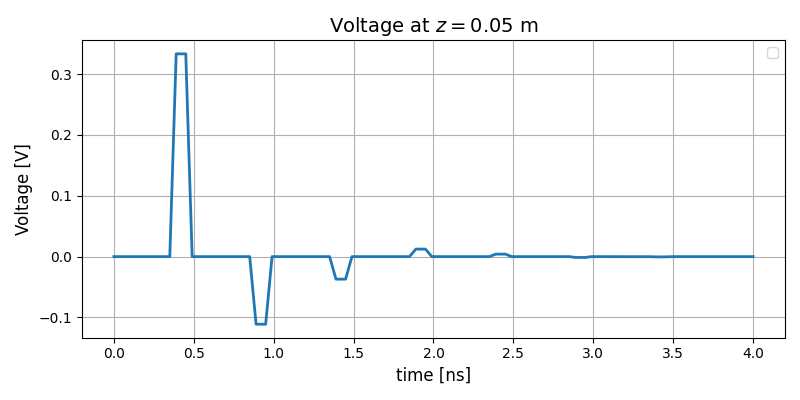
\includegraphics[scale=0.5]{figures/default.png}
    \caption{Bit behavior (voltage profile) under default settings}
    \label{fig:default}
\end{figure}

When $\tau_h$ becomes larger than 0.5 nanoseconds, interference between incident and reflected bits occur. The zero parts on the graph (in function of time) disappear and incidences and reflections influence each other, either positive or negative interference. This effect is shown in figure~\ref{fig:TH}.

\begin{figure}[h!]
    \centering
    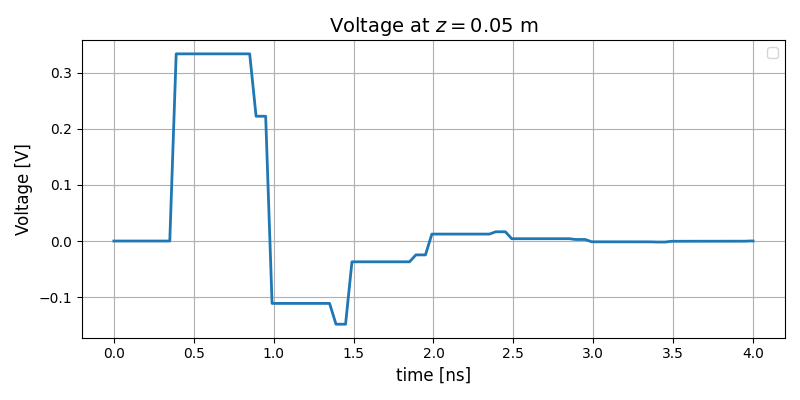
\includegraphics[scale=0.5]{figures/tau_h=0.5ns.png}
    \caption{$\tau_h = 500*10^{-12}$}
    \label{fig:TH}
\end{figure}

In the case of $\tau_h = \tau_r$, the bit has a triangular shape, as shown in figure~\ref{fig:sub1}. A curious effect can be noticed in the voltage profile when $\tau_r$ approaches 0. One would expect the bit to have square wave shape, but instead some non converging effects occur displayed in figure~\ref{fig:sub2}.

\begin{figure}[! h]
\centering
\begin{subfigure}{.5\textwidth}
  \centering
  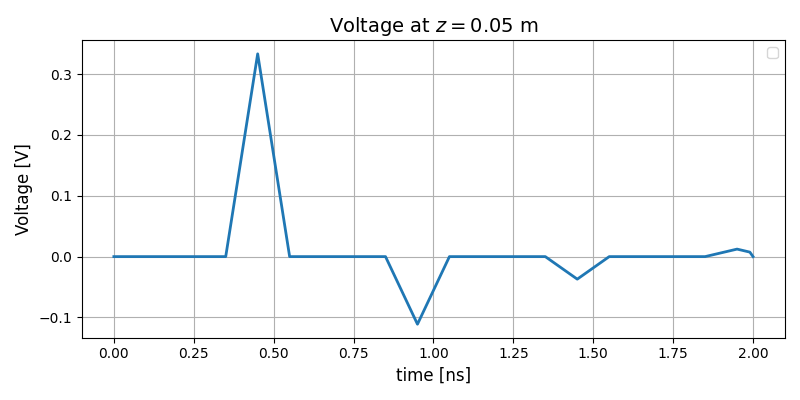
\includegraphics[width=.9\linewidth]{figures/tau_h_equals_tau_r.png}
  \caption{$\tau_h = \tau_r$}
  \label{fig:sub1}
\end{subfigure}%
\begin{subfigure}{.5\textwidth}
  \centering
  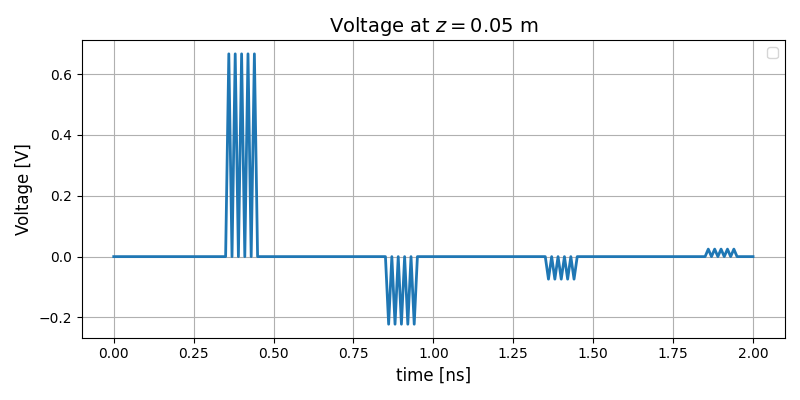
\includegraphics[width=.9\linewidth]{figures/tau_r naar 0.png}
  \caption{$\tau_r = 10^{-12}$}
  \label{fig:sub2}
\end{subfigure}
\caption{}
\label{fig:test}
\end{figure}